\section{Microscopic Pedestrian Model}

We will first construct the pedestrian model focusing on the interaction of agents to each other i.e. in the microscopic scale. In contrast, the macroscopic scale would focus on the resulting dynamics of the agents' interactions as a collective, which will be presented in more detail in the next section.

\subsection{Pedestrian Attributes}
Let us first start by describing our model. We follow the approach presented in \cite{tordeux2022multi} which follows a general class of microscopic force-based models approach given in \cite{helbing1995social,chraibi2011force}. The pedestrians exist on a toroidal surface, in other words, our model has periodic boundaries. For simplicity, the mass for all pedestrians is set to 1, hence their momentum $p_i$ is equal to the velocity, i.e. $p_i = m_i v_i = v_i$. The pedestrians also posses a desired velocity, which is assigned to each of them as an input to the model, this directs the pedestrians to desire a certain direction to move towards during the simulation run.

Given a pedestrian $i$ in $\mathbb{R}^2$ and time $0\leq t \leq T$, it possesses the following attributes:
\begin{itemize}
    \item Desired velocity: $u_i(t): [0,T] \mapsto \mathbb{R}^2$ 
    \item Current velocity: $p_i(t): [0,T] \mapsto \mathbb{R}^2$
    \item Current position: $q_i(t): [0,T] \mapsto \mathbb{R}^2$
\end{itemize} 
\begin{listing}[!ht]
\begin{minted}[escapeinside=??, frame=single]{julia}
## Define Agent
using Agents
@agent struct Pedestrian(ContinuousAgent{2,Float64})
    u?\sub{i}?::Vector{Float64} # Desired Velocity
end
\end{minted}
\caption{Defining the pedestrian agent in Julia's Agents.jl package. It is to be noted that \texttt{ContinuousAgent} specifies that our Pedestrian is a continuous agent with predefined position and velocity attributes constructed within the \texttt{@agent} macro. We only need to declare additional attributes such as \texttt{u}\sub{i}} 
\label{code:agent_def}
\end{listing}

For a model with $N \geq 2$ pedestrians, the relative position $\dot Q_{ij}(t)$ of a pedestrian $i$ to pedestrian $j$ is denoted as follows
\begin{align*}
    {Q}_{ij}(t) = q_i - q_j
\end{align*}
The vector of relative positions $Q_i(t)$ of a pedestrian $i$ to all pedestrians $j \neq i$ is denoted as follows
\begin{align*}
    {Q}_{i}(t) = ({Q}_{ij}(t))_{i\neq j} : [0,T] \mapsto \mathbb{R}^{2\cdot(N-1)} \text{ for } j = 1,\dots, N, \quad j \neq i
\end{align*}


\subsection{Microscopic Model Dynamics}
\label{section:micro_model_dynamics}
The dynamics of the pedestrians are based on (i) short-range repulsion $U$ among pedestrians based on their distances from others and (ii) attraction $\lambda$ toward a desired velocity $u_i$. The microscopic dynamics for the pedestrian $i$ is given by the following equations:
\begin{equation}
\begin{aligned}
    \dot Q_{ij}(t) &= p_i(t) - p_j(t), &j = 1,\dots,N \quad j \neq i& & \dot Q_i(0) &= Q^0_i \\
    \dot p_i(t) &= \lambda(u_i(t) - p_i(t)) - \sum_{j \neq i} \nabla U (Q_{ij}(t)), && & \dot p_i(0) &= p^0_i
\end{aligned}
\label{eq:micro}
\end{equation}
Here,
\begin{itemize}
    \item $\lambda \in \mathbb{R}_{\geq 0}$, is a parameter for the relaxation rate. In other words, it determines the intensity to reach the desired velocity. 
    \item $U(Q_{ij})$, is a nonlinear repulsive interaction potential, such that it is always positive and convex. This determines the magnitude of repulsion of a pedestrian $i$ to other pedestrians $j$ as a function of relative position $Q_{ij} = q_i - q_j$. It is defined as follows 
    \begin{align} 
        U(x) : \mathbb{R}^2 \mapsto \mathbb{R}, \quad\quad U(x) = ABe^{-|x|/B}
        \label{eq:def_potU}
    \end{align}
    Here, $|\cdot|$ is the minimum euclidean distance on the torus. $A$ and $B$ are scalar-valued parameters for the repulsion strength and the range of interaction respectively.
\end{itemize}

Hence, $\nabla U(x):\mathbb{R}^2 \mapsto \mathbb{R}^2$ is defined as
\begin{align} 
    \nabla U(x) = -A\dfrac{x}{|x|}e^{-|x|/B} = -\nabla U(-x)
    \label{eq:def_U}
\end{align}
It can be seen that this parameter is responsible for avoiding collisions between pedestrians, ensuring that the repulsive forces increase in magnitude the closer a pedestrian is. The underlying assumption is that the repulsive forces are a function of distance only. This is adapted from the concept of social forces and how they are determined from the surroundings of pedestrians.

Using the product rule, the Hessian $\mathbf{H}_U = \nabla ^2 U(x):\mathbb{R}^2 \mapsto \mathbb{R}^{2\times2}$ can be expressed as:
\begin{align}
    \mathbf{H}_U &= \nabla^2 U(x) = -A\left(\dfrac{x}{|x|}\dfrac{\d}{\d x} \left[ e^{-|x|/B} \right] + e^{-|x|/B}\dfrac{\d}{\d x} \left[\dfrac{x}{|x|}\right]\right) \nonumber \\ 
    &= \nabla^2 U(x) = -A\left[\dfrac{1}{|x|}\left(I - \dfrac{xx^T}{|x|^2}\right) - \dfrac{1}{B}\dfrac{xx^T}{|x|^2}\right]e^{-|x|/B}
    \label{eq:def_ddU}
\end{align}

Which will be used to evaluate the stochastic derivative in \autoref{section:stoch_derivative}

\subsection{Stochastic Model Dynamics}

To study the stochastic variant of our model, and how they effect the overall dynamics, we will introduce stochastic terms into our model. Generally a typical stochastic differential equation (SDE) is of the form
\begin{equation*}
    \d X_t = \underbrace{f(X_t, t)\d t}_{\text{drift}} + \underbrace{g(X_t, t)\d W_t}_{\text{diffusion}}
\end{equation*}
Which is a combination of a deterministic component, denoted as the \textit{drift} term; and a stochastic component, denoted as the \textit{diffusion} term. In our case, we introduce an additive noise term $\sigma dW_i(t)$ to our deterministic model from before \autoref{eq:micro} resulting in \autoref{eq:stoch_micro}. To be able to have a better physical interpretation of the model, the noise is introduced in the momentum term, rather than the position term. So one can interpret this as agents moving randomly while maintaining a continuous motion, as opposed to randomly teleporting in different locations at every time-step.
\begin{gather}
\begin{aligned}
    \d Q_{ij}(t) &= (p_i(t) - p_j(t))\d t \\
    \d p_i(t) &= \lambda(u_i(t) - p_i(t))\d t - \sum_{j \neq i} \nabla U (Q_{ij}(t))\d t + \sigma \d W_i(t)
    \label{eq:stoch_micro}
\end{aligned}
\end{gather}

The equation is reminiscent of a typical SDE with the first two terms being the deterministic part of the equation, i.e. drift and the last term being the stochastic part, i.e. the diffusion term. The randomness is induced via the Wiener process $(W_i(t))^N_{i=1}: [0,\infty) \times \Omega \rightarrow \mathbb{R}^N$, which is a mathematical description of the Brownian motion, that generates a sequence of random variables defined on a probability space $(\Omega, F, P)$ with independent increments \cite{oksendal2003stochastic}. Here, $\Omega$ is the sample space, $F$ the event space, and $P$ the probability measure. The stochastic term is amplified by the constant $\sigma \in \mathbb{R}$, which is often denoted as the volatility or diffusion coefficient.


\subsection{Identifying Collective Phenomenon}
With the dynamics presented so far, we can observe the individual pedestrian's attributes change over time. However, to identify whether a collective phenomenon is occurring we have also constructed a simple formula to measure the mean direction of all agents relative to their desired velocity direction, i.e. direction alignment.

To measure how much an agent $i$ is moving in the direction of its particular desired velocity $u_i$, we can take the following dot product.
\begin{gather}
    \text{Alignment}_i = \dfrac{p_i}{|p_i|} \cdot \dfrac{u_i}{|u_i|}
\end{gather}
The range of this measure is $[-1, 1]$, with 1 indicating that the pedestrian is moving exactly in its desired direction, -1 indicating that the pedestrian is moving exactly opposite to its desired direction, whereas 0 indicates that it is either not moving or it is moving perpendicular to its desired speed. We can use this measure to quantify the mean direction of all agents. In other words, how aligned the mean direction of all agents is to their desired direction.
\begin{align}
    \text{Alignment} &= \dfrac{1}{N}\sum_{i=1}^N \text{Alignment}_i \nonumber \\
    &= \dfrac{1}{N}\hat p^T \hat u
    \label{eq:alignment}
\end{align}
This will be useful, as we will later see, in identifying ordered and disordered collective dynamics. From a collective point of view, we can say that the value near 1 or -1 will indicate orderly behavior, signalling that all pedestrians are moving in their respective desired directions. Whereas values near 0 will indicate disorder.

\textbf{Calculation of Alignment}

In our simulations, we can take advantage of the fact that $u_i$ is always going to be a unit vector, i.e. either $[1,0]$, $[0,1]$, or $[0,0]$. Thus, we only use the unit vector of the velocity in the calculation of the alignment from \autoref{eq:alignment}, as shown in the code below.

\begin{listing}[H]
\begin{minted}[escapeinside=@@, frame=single, fontsize=\small]{julia}    
function calc_alignment(model)
    return mean(
        [transpose(i.vel/norm(i.vel))*(i.@u\sub{i}@) for i in allagents(model)]
        )
end
\end{minted}
\caption{Calculation of Mean direction of all pedestrians}
\label{code:calc_alignment}
\end{listing}

The benefit of this measure is made apparent in \autoref{plot:align_uni}. Here, we see how the mean direction of all the pedestrians gradually aligns with their desired velocity direction as the value moves from 0 to 1, showing the presence of order in the system.
\begin{figure}[H]
    \centering
    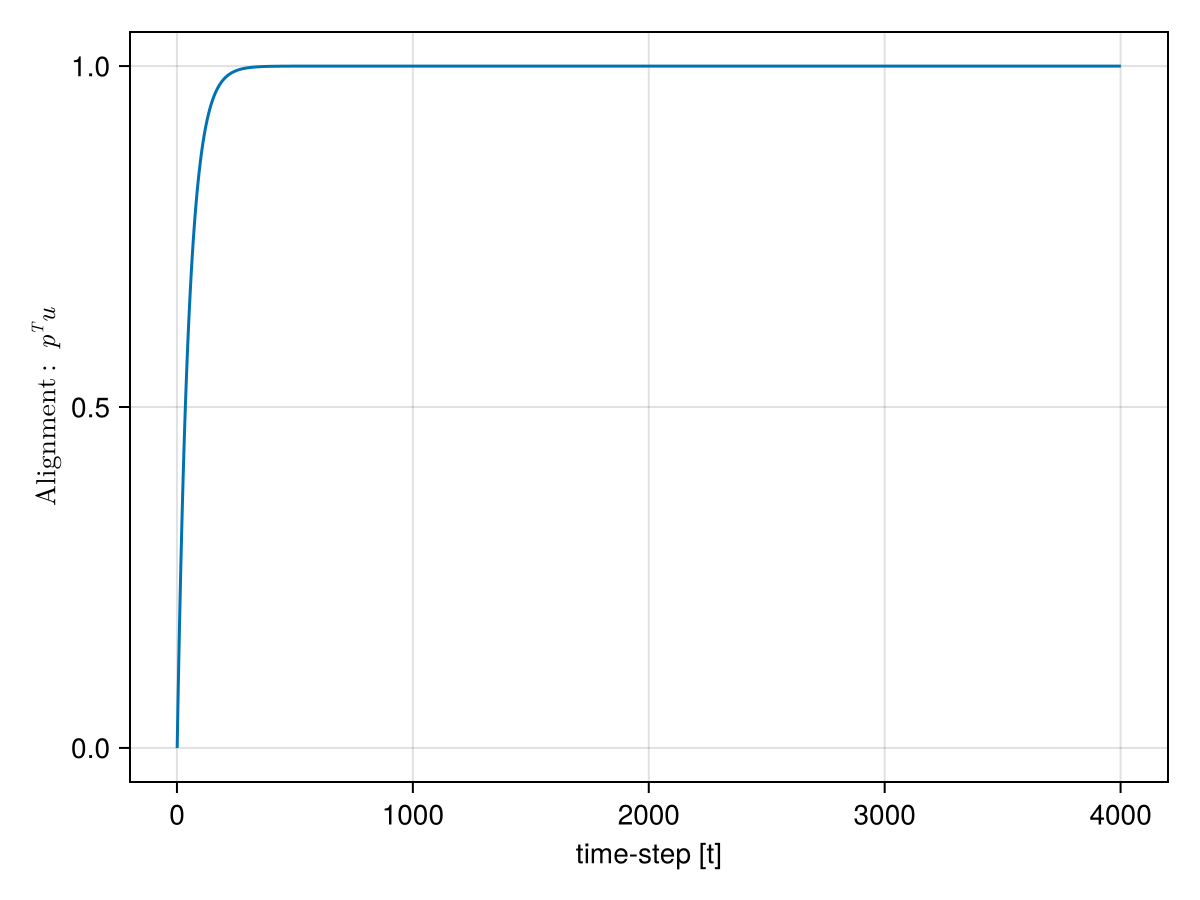
\includegraphics[width=0.49\linewidth]{figures/ch4_uniflow/straight_uni.png}
    \caption{Alignment for unidirectional flow.}
    \label{plot:align_uni}
\end{figure}

Through this measure, we can witness a shift from order to disorder by means of pedestrians aligning with their respective desired direction. Examples of this with various other cases will be shown in \autoref{section:observations}.